% !TEX root = ../main.tex
\documentclass[../main.tex]{subfiles}
\begin{document}

\section{Mathematical description of the poly-line separation measure}
\label{appendix:clustering_maths}

This appendix details the metric used in Section \ref{sec:aggregation_of_volunteer_models} to cluster poly\-lines used by volunteers to model spirals arms. It can be seen as a variant of the Fréchet distance. The metric is illustrated in Figure \ref{fig:spiral_metric_description}.

\begin{figure}
  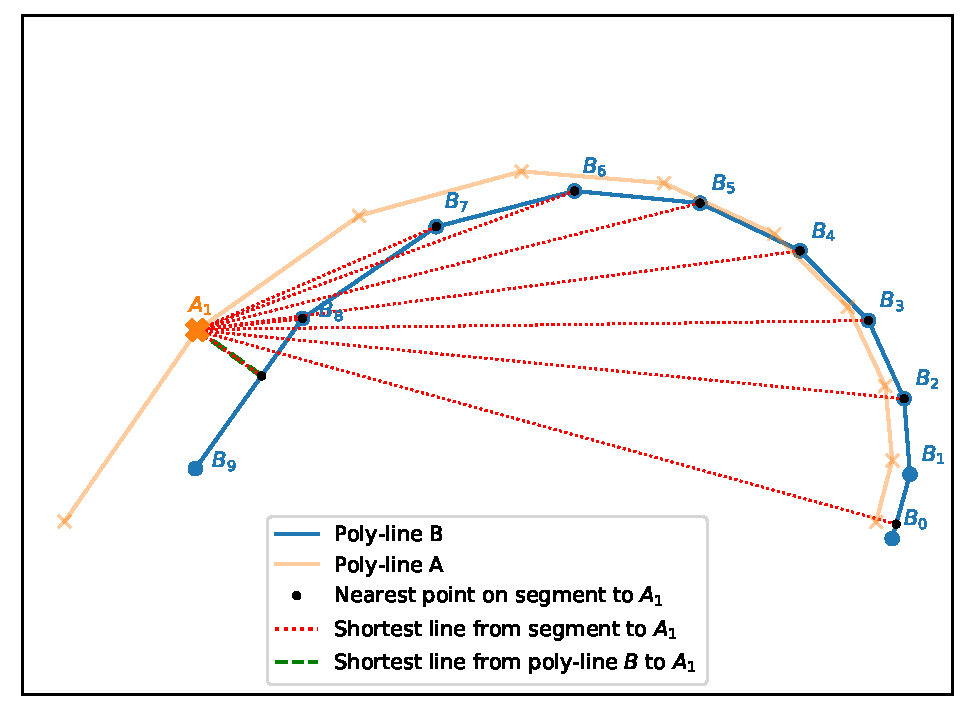
\includegraphics[width=8cm]{images__appendix/spiral_metric_description.pdf}
  \caption{Illustration of the metric used. For each point in line $A$, the shortest distance to each segment in line $B$ is calculated (shown as dotted red lines). The minimum of these distances (corresponding to the line shown in dashed green) is squared.}
  \label{fig:spiral_metric_description}
\end{figure}

First, define a poly-line containing $n$ 2D cartesian coordinates (vertices) as

\begin{equation}
A: \{i \in \mathbb{N};\;i<n\} \longrightarrow \mathbb{R}
^2\end{equation}

We also define a function, $t$, which calculates how far a point $\vec{p}$ is along the line between two other points ($\vec{v}$ and $\vec{w}$):

\begin{equation}
t(\vec{p},\,\vec{v},\,\vec{w}) \equiv \frac{(\vec{p} - \vec{v})\cdot(\vec{v} - \vec{w})}{|\vec{w} - \vec{v}|^2}.
\end{equation}

The minimum distance from $\vec{p}$ to the line segment between $\vec{v}$ and $\vec{w}$ is given by

\begin{equation}
d(\vec{p},\,\vec{v},\,\vec{w}) = \|\left(\vec{v} + \mathrm{min}(\mathrm{max}(t(\vec{p},\,\vec{v},\,\vec{w}),\, 0),\, 1)\;(\vec{w} - \vec{v})\right) - \vec{p}\|
\end{equation}

We then define a ``squared distance'' from the poly-line $A$ (containing $n$ vertices) to the poly-line $B$ (containing $m$ vertices):

\begin{equation}
D(A,\,B) \equiv \frac{1}{n}\sum_{i = 0}^{n} \mathrm{min}\{j \in \mathbb{N}_0,\, j < m;\; d(A_i,\, B_j,\, B_{j+1})^2\}.
\end{equation}

The choice to square the distances and penalize large deviations from other lines was a data-driven choice to improve the results of clustering.

Finally, we define our separation measure between two drawn poly-lines as

\begin{equation}
distance(A,\,B) \equiv D(A,\,B) + D(B,\,A).
\end{equation}


\section{Stacking of multiple SDSS Frames}
\label{appendix:frame_stacking}

 All data required for sigma image creation for stacked frames came from the corrected frames, as detailed in the frame datamodel\footnote{\url{https://data.sdss.org/datamodel/files/BOSS_PHOTOOBJ/frames/RERUN/RUN/CAMCOL/frame.html\#example}}. For each pixel in an SDSS frame, we have

\begin{equation}
\frac{I}{C} = \frac{n}{g} - S + V,
\end{equation}

where $I$ represents the sky-subtracted, corrected image (nanomaggies), $C$ reprents the calibration image, $n$ is the number of electrons captured, $g$ is the gain, $S$ is the Sky value (data units) and $V$ is the dark current, $V = 0 ± \sqrt{v}$ ($v$ being the dark variance).

Given Poisson error,

\begin{equation}
\sigma_n = \sqrt{n}.
\end{equation}

If we stack multiple frames, given $N$ observations of a pixel

\begin{equation}
  \begin{aligned}
n_\mathrm{total} &= \sum_i{n_i} = \sum_i g_i\left(\frac{I_i}{C_i} + S_i - V_i\right),\\
                 &= \sum_{i}\frac{g_i}{C_i}I_i + \sum_i{g_i \left(S_i - V_i\right)} = \sigma_{n_\mathrm{total}}^2.
  \end{aligned}
\end{equation}

This is ideal, and is the level that many fitting software packages work at, we, however, want to return to working in units of nanomaggies on a stacked image, and so further calculation is needed:

\begin{equation}
I = \frac{1}{N}\sum_i I_i,
\end{equation}

\begin{equation}
I = \frac{1}{N}\sum_i C_i\left(\frac{n_i}{g_i} - S_i + V_i\right),
\end{equation}

And so

\begin{equation}
  \sigma_I^2 = \frac{1}{N^2}\sum_i\frac{C_i^2}{g_i^2}\sigma_{n_i}^2 + \frac{1}{N^2}\sum_i C_i^2 \sigma_{S_i}^2 + \frac{1}{N^2}\sum_i C_i^2 \sigma_{V_i}^2.
\end{equation}

We treat the sky value as a constant, such that $\sigma_{S_i}^2 = 0$. Substituting $\sigma_{n_i}^2 = n_i$ as above gives

\begin{equation}
  \sigma_I^2 = \frac{1}{N^2}\sum_i\frac{C_i^2}{g_i^2}n_i + \frac{1}{N^2}\sum_i C_i^2 v_i.
\end{equation}

\begin{equation}
  \sigma_I = \frac{1}{N}\sqrt{\sum_i C_i^2\left(\frac{n_i}{g_i^2} + v_i\right)}.
\end{equation}
Note that this is identical to saying

\begin{equation}
\sigma_I^2 = \frac{1}{N^2}\sum_i\sigma_{I_i}^2.
\end{equation}

\section{Ancillary Tables}
\begin{table*}
  \centering
  \caption{The maximum, minimum and default values for model parameters. Note that some parameters were allowed to overflow when fitting, for instance an axis ratio greater 1 (signifying a swap of major and minor axis) was allowed, and corrected for once fitting reached completion. This helped avoid the optimizer encountering parameter bounds and failing to converge. Component roll was similarly unconstrained.}
  \begin{tabular}{l|l|r|r|r|r|r}
\hline
Component & Parameter  & Tuning Minimum & Tuning Maximum \\
          &            &  Bound         & Bound          \\
\hline
disc      & $\mu_x$    & -inf           & inf            \\
          & $\mu_y$    & -inf           & inf            \\
          & roll       & -inf           & inf            \\
          & $q$        & 0.01           & 100            \\
          & $R_e$      & 0              & inf            \\
          & $\Sigma_e$ & 0              & inf            \\
bulge     & $\mu_x$    & -inf           & inf            \\
          & $\mu_y$    & -inf           & inf            \\
          & roll       & -inf           & inf            \\
          & $q$        & 0.01           & 100            \\
          & $R_e$      & 0              & inf            \\
          & $\Sigma_e$ & 0              & inf            \\
          & $n$        & 0.1            & 10             \\
bar       & $\mu_x$    & -inf           & inf            \\
          & $\mu_y$    & -inf           & inf            \\
          & roll       & -inf           & inf            \\
          & $q$        & 0.01           & 100            \\
          & $R_e$      & 0              & inf            \\
          & $\Sigma_e$ & 0              & inf            \\
          & $n$        & 0.1            & 10             \\
          & $c$        & 0.01           & 10             \\
spiral    & $\Sigma_e$ & 0              & inf            \\
          & spread     & 0              & inf            \\
          & falloff    & 0.01           & inf            \\
\hline
  \centering
  \end{tabular}
  \label{table:bad_values}
\end{table*}

\begin{table*}
  \centering
  \caption{Pivot table of reported errors on parameters for our sample of 297 galaxies. Errors quoted are absolute errors.}
  \begin{tabular}{l|l|rrrrrrrr}
  \hline
  component & parameter &  count &  mean &   std &   min &   25\% &   50\% &   75\% &    max \\
  \hline
  disk  & $\Sigma_e$ (nmgy) &    291 &  0.20 &  0.21 &  0.01 &  0.07 &  0.14 &  0.25 &  1.22 \\
        & $r_e$ &    291 &  0.65 &  0.32 &  0.08 &  0.42 &  0.60 &  0.85 &  1.82 \\
        & $\mu_x$ (arcseconds) &    291 &  0.43 &  0.28 &  0.05 &  0.24 &  0.38 &  0.56 &  2.56 \\
        & $\mu_y$ (arcseconds) &    291 &  0.44 &  0.26 &  0.11 &  0.26 &  0.36 &  0.54 &  1.93 \\
        & $b/a$ &    291 &  0.09 &  0.04 &  0.01 &  0.06 &  0.09 &  0.12 &  0.20 \\
        & $\phi$ (radians) &    291 &  1.63 &  0.36 &  0.21 &  1.43 &  1.58 &  1.77 &  2.93 \\
  bulge & $\Sigma_e$ (nmgy) &    272 &  0.75 &  0.96 &  0.00 &  0.16 &  0.39 &  0.85 &  6.75 \\
        & $r_e$ &    272 &  0.08 &  0.05 &  0.00 &  0.05 &  0.07 &  0.10 &  0.47 \\
        & $\mu_x$ (arcseconds) &    272 &  0.13 &  0.08 &  0.00 &  0.09 &  0.12 &  0.16 &  0.72 \\
        & $\mu_y$ (arcseconds) &    272 &  0.13 &  0.07 &  0.00 &  0.09 &  0.11 &  0.16 &  0.51 \\
        & $n$ &    272 &  1.23 &  0.64 &  0.00 &  0.63 &  1.40 &  1.73 &  2.48 \\
        & $b/a$ &    272 &  0.10 &  0.05 &  0.00 &  0.07 &  0.10 &  0.14 &  0.23 \\
        & $\phi$ (radians) &    272 &  1.56 &  0.57 &  0.00 &  1.28 &  1.57 &  1.86 &  3.47 \\
  bar   & $\Sigma_e$ (nmgy) &     92 &  0.31 &  0.39 &  0.00 &  0.06 &  0.16 &  0.39 &  2.36 \\
        & $r_e$ &     92 &  0.16 &  0.12 &  0.02 &  0.06 &  0.14 &  0.20 &  0.87 \\
        & $c$ &     92 &  0.28 &  0.20 &  0.00 &  0.14 &  0.25 &  0.42 &  0.82 \\
        & $\mu_x$ (arcseconds) &     92 &  0.23 &  0.26 &  0.04 &  0.11 &  0.17 &  0.27 &  2.24 \\
        & $\mu_y$ (arcseconds) &     92 &  0.24 &  0.20 &  0.02 &  0.13 &  0.18 &  0.31 &  1.09 \\
        & $n$ &     92 &  0.37 &  0.30 &  0.00 &  0.08 &  0.30 &  0.66 &  0.88 \\
        & $b/a$ &     92 &  0.09 &  0.04 &  0.01 &  0.06 &  0.08 &  0.11 &  0.23 \\
        & $\phi$ (radians) &     92 &  0.69 &  0.98 &  0.00 &  0.06 &  0.10 &  1.17 &  3.57 \\
  \hline
  \end{tabular}
  \label{table:error_values}
\end{table*}
\end{document}
